% DUNE experiment
% Target length: 25 pages

\graphicspath{{DUNE/Figs/}}

\chapter{The Deep Underground Neutrino Experiment}\label{chap:DUNE}

The Deep Underground Neutrino Experiment (DUNE) experiment \cite{DUNECDR1,DUNECDR2,DUNECDR3,DUNECDR4} is a future long-baseline neutrino experiment with a diverse physics program hosted by Fermilab, IL, U.S..  The far detector will be at the Sanford Underground Research Facility (SURF) near Lead, South Dakota, providing a baseline of 1300~km.  A cartoon of the experiment is shown in Figure~\ref{fig:DUNE}.

\begin{figure}
  \centering
  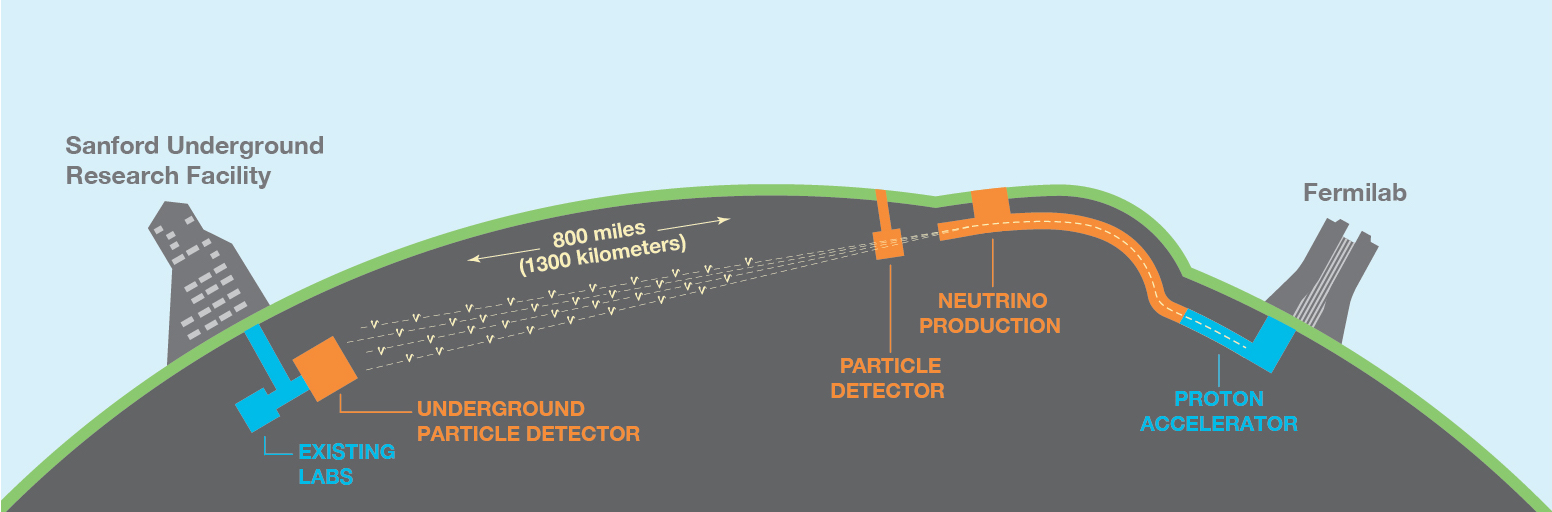
\includegraphics[width=14cm]{DUNE.jpg}
  \caption[Cartoon showing the configuration of the Deep Underground Neutrino Experiment.]{Cartoon showing the configuratuon of the Deep Underground Neutrino Experiment.  The experiment will be based at Fermilab, shown at the right of the figure, and will send neutrinos towards SURF, at the left hand side.  The distance travelled, through the Earth's crust, will be 1300~km.}
  \label{fig:DUNE}
\end{figure}

The DUNE experiment will be discussed in this present chapter.  As the experiment utilises liquid argon TPCs, a brief history and description of this detector technology is provided as a basis in Section~\ref{sec:LArTPC}.  An overview of the experiment, including its motivation, will be presented in Section~\ref{sec:DUNEOverview} before the experimental details are discussed in Section~\ref{sec:DUNEExperiment}.  The sensitivities of the experiment and its potential discoveries are the subject of Section~\ref{sec:DUNEPhysics}.  Finally, the schedule and stategy implemented by the collaboration to ensure commencement of data taking in around ten years' time is outlined in Section~\ref{sec:RoadToDUNE}.

%----------------------------------------------------------------------------------------------------------------------------------------------------------------------------
\section{The LAr TPC Concept}\label{sec:LArTPC}

The use of a liquid argon time projection chamber (LArTPC) as a high-precision fine-grained detector medium holds much promise for the successful resolution of the open questions in neutrino physics.  A great amount of R\&D work has taken place to advance the maturity of the technology and pioneering experiments, such as ICARUS \cite{ICARUS2004}, have further increased the understanding of the neutrino community of the detector techniques.  Past and currently running experiments at Fermilab, such as ArgoNeuT \cite{ArgoNeuT2012}, LArIAT \cite{LArIAT2014} and MicroBooNE \cite{MicroBooNE2017}, are successfully using LArTPCs to take and analyse data and it seems certain to be the future of neutrino physics in the U.S. \cite{Baller2014}.

This section will provide a brief history of LArTPC technology and motivate its potential when used in a large experiment such as DUNE.  The basic operation of such a detector will also be described to provide background for discussion of the DUNE and 35~ton experiments, and of reconstruction in LArTPCs, in future chapters.

%----------------------------------------------------------------------------------------------------------------------------------------------------------------------------
\subsection{A Brief History of Time (Projection Chambers)}\label{sec:LArTPCHistory}

The use of a time projection chamber as a potential particle detector was put forward by David Nygren in 1974 \cite{Nygren1974}.  He envisioned bubble-chamber quality data but with the possibility of digital readout of the data, facilitating extremely fine spatial resolution, good timing resolution and fast recovery after triggering.  The basic concept is a drift chamber containing a noble gas placed within a field to drift ionisation electrons created by a propagating particle towards a multielectron array.  This setup allows full three-dimensional reconstruction by combining information from the two-dimensional readout plane with the drift time.  Nygren also included a magnetic field to assist particle identification in his design, shown in Figure~\ref{fig:NygrenTPC}.

\begin{figure}
  \centering
  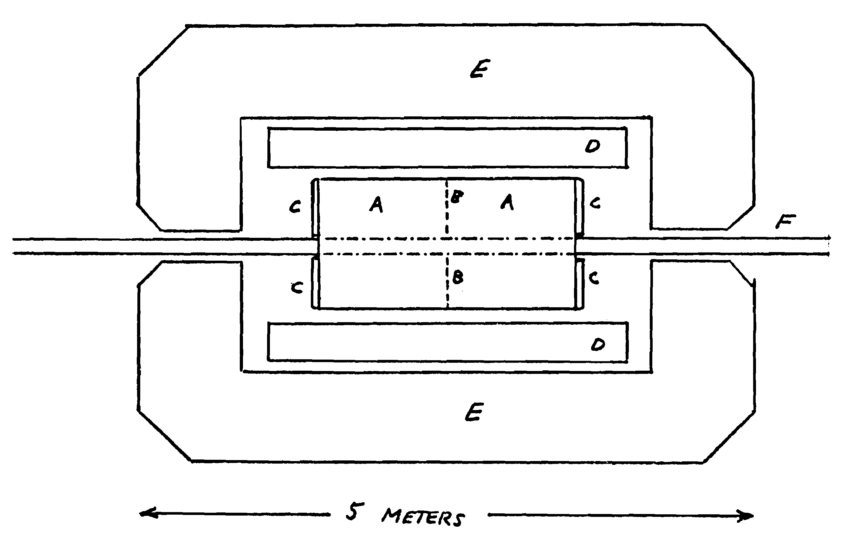
\includegraphics[width=10cm]{NygrenTPC.png}
  \caption[Original TPC design, Nygren (1974)]{The original concept of the time projection chamber particle detector, drawn by David Nygren in 1974 \cite{Nygren1974}.  The sections are labelled as followed: methane-filled region (A), screen to establish electron field (B), end-cap detectors (C), superconducting solenoid (3.33~T) (D), iron return yoke for magnetic field (E), beam vacuum pipe (F).}
  \label{fig:NygrenTPC}
\end{figure}

The extension of this concept to a liquid argon TPC and its potential as a high-precision fine-grained detector medium in neutrino physics was proposed by Carlo Rubbia in 1977 \cite{Rubbia1977}.  The use of a noble liquid rather than gas is necessary in neutrino experiments to provide a high enough target mass for increased probability of neutrino interactions.  Noble liquids have high electron mobility and low diffusion, favourable properties as the detection of particles is from the ionisation and scintillation light created by the particles.  Given the necessity of a high electric field in order to drift these electrons to the readout places, excellent dielectric properties are also required; noble liquids possess such qualities.  The properties of liquid argon which make it almost perfect for this use are demonstrated in Table~\ref{tab:NobleProperties}.

\begin{table}
  \caption{Properties of noble liquids relevant when considering a TPC medium for a neutrino experiment \cite{Soderberg2008}.}
  \label{tab:NobleProperties}
  \centering
  \begin{tabular}{ l c c c c c c }
    \toprule
     & Water & He & Ne & \color{red} Ar & Kr & Xe \\
    \midrule
    Boiling point [K] @ 1 atm & 373 & 4.2 & 27.1 & \color{red} 87.3 & 120.0 & 165.0 \\
    Density [g/cm$^3$] & 1 & 0.125 & 1.2 & \color{red} 1.4 & 2.4 & 3.0 \\
    Radiation length [cm] & 36.1 & 755.2 & 24.0 & \color{red} 14.0 & 4.9 & 2.8 \\
    Scintillation [$\gamma$/MeV] & - & 19 000 & 30 000 & \color{red} 40 000 & 25 000 & 42 000 \\
    dE/dx [MeV/cm] & 1.9 & 0.24 & 1.4 & \color{red} 2.1 & 3.0 & 3.8 \\
    Scintillation $\lambda$ [nm] & - & 80 & 78 & \color{red} 128 & 150 & 175 \\
    Abundance (Earth atm) [ppm] & $5\times 10^4$ & 5.2 & 18.2 & \color{red} 9340.0 & 1.10 & 0.09 \\
    Electron mobility [cm$^2$/Vs] & low & low & low & \color{red} 400 & 1200 & 2200 \\
    \bottomrule
  \end{tabular}
\end{table}

An additional advantage of this technology is the low threshold for detection; this is set by the ionisation threshold of liquid argon and is only $23.6 \pm 0.5$ eV \cite{Chepel2013}.  Rubbia realised that a LArTPC could be the digital replacement for the high quality particle detection methods used in bubble chambers, very common in neutrino physics in the 1970s.  He proposed the first LArTPC detector design, shown in Figure~\ref{fig:RubbiaLArTPC}, which bears a striking resemblance to the LArTPCs in use today.

\begin{figure}
  \centering
  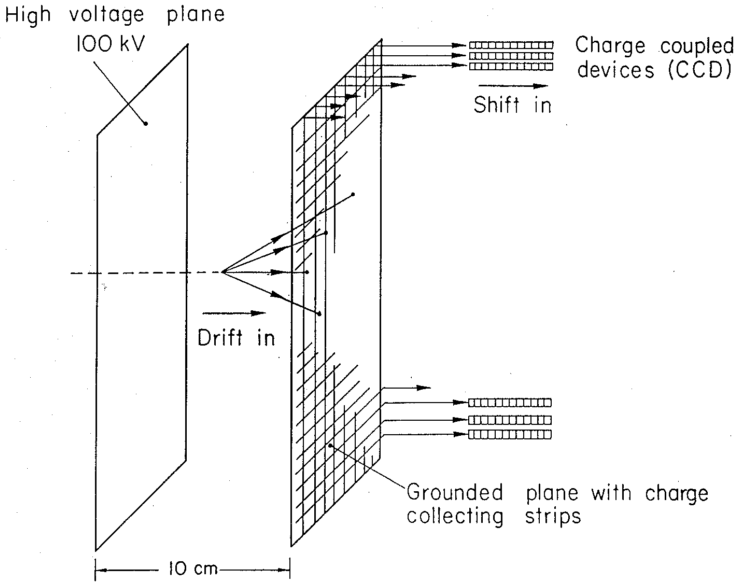
\includegraphics[width=10cm]{RubbiaLArTPC.png}
  \caption[First LArTPC detector, Rubbia (1977)]{The LArTPC detector proposed by Carlo Rubbia in 1977 \cite{Rubbia1977}.}
  \label{fig:RubbiaLArTPC}
\end{figure}

Constructing and operating such a detector was beyond the technology of the time, and is still being understood today.  The operation of a LArTPC detector and the challenges associated with this are the subject of Section~\ref{sec:LArTPCOperation}.

%----------------------------------------------------------------------------------------------------------------------------------------------------------------------------
\subsection{LAr TPC Operation}\label{sec:LArTPCOperation}

A LArTPC typically consists of one or more anodes and cathodes at either end of an active drift region.  An ionising particle passing through a LArTPC causes electrons to become free from argon atoms and, in the presence of a field, drift towards an anode where they are read out.

The readout consists of multiple wire planes with different orientations to facilitate the reconstruction.  The wires are either `induction' wires, which allow the electrons to deposit charge but continue past, or `collection' wires, on which the electric field lines end and all the charge on the electron is collected.  Each wire plane is therefore held at a different `bias voltage' to prevent any field lines ending on the induction wire, thus creating local electric fields which promote the continuing forward motion of the electrons.  The signal seen is therefore dependent on the type of wire plane; a bipolar pulse on an induction plane wire and unipolar on a collection plane wire.  It is also common, though not essential, to make use of a `grid plane' upstream of the signal planes in order to shield them from the electron charge until the drift electrons are close.  Without such a plane, the bipolar pulse would be highly asymmetric, though would still have zero integral.  It also makes changing the drift voltage (controlling the electric field) slightly easier as the signal planes are somewhat shielded from its effects.  MicroBooNE does not operate with a grid plane and, although the 35~ton and the DUNE reference design make use of a grid plane, it is uncertain whether the benefit outweighs the cost for a huge LArTPC detector such as the DUNE far detector.  There are alternative readout possibilities to this typical design which have been suggested but, given the scale of future LArTPCs, it is highly unlikely a viable solution which delivers superior readout at a comparable cost will be found.

Upon ionisation, an electron has a certain probability (around 60\%) of recombining before the field can separate it from its ion.  Whilst this compromises the signal observed, it is accompanied by a flash of scintillation light which may be detected and used to assign an `event time' to the interaction, known as T0.  Without this information, it would be impossible to place an absolute time scale on the event and result in an unresolved coordinate along the drift direction.  The magnitude of the applied electric field must be chosen to balance these two effects; a larger field would result in less recombination and therefore compromise the scintillation light while a smaller field would have consequences on the signal received at the wire planes.  Figure~\ref{fig:ElectricFieldScintillationIonisation} demonstrates this and justifies the field value of 500~V/cm which is often chosen in current LAr neutrino experiments.

\begin{figure}
  \centering
  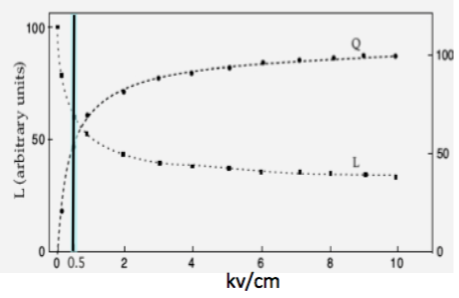
\includegraphics[width=12cm]{ElectricFieldScintillationIonisation.png}
  \caption[Effect of electric field on luminosity of ionisation electrons and scintillation light in a LArTPC.]{Demonstration of the competing effect the electric field has on the luminosity of the ionisation electrons and scintillation light arriving at the detector readout.  Since both are essential in reconstructing the complete interactions, a balance must be found. [PLACEHOLDER IMAGE].}
  \label{fig:ElectricFieldScintillationIonisation}
\end{figure}

The basic operational principles of a LArTPC is demonstrated in Figure~\ref{fig:LArTPCOperation}.  The specifics of how the ionisation charge and the scintillation light is collected and processed is experiment-specific and will be discussed in the context of DUNE in Chapter \ref{chap:DUNE} and the 35~ton experiment in Chapter \ref{chap:35ton}.  This information is all that is required to fully understand and analyse the interactions occurring in the detector; methods used to reconstruct particles and interactions in LAr will be the subject of Chapter \ref{chap:LArTPCReconstruction}.

\begin{figure}[p]
  \centering
  \begin{subfigure}[t]{0.48\linewidth}
    \centering
    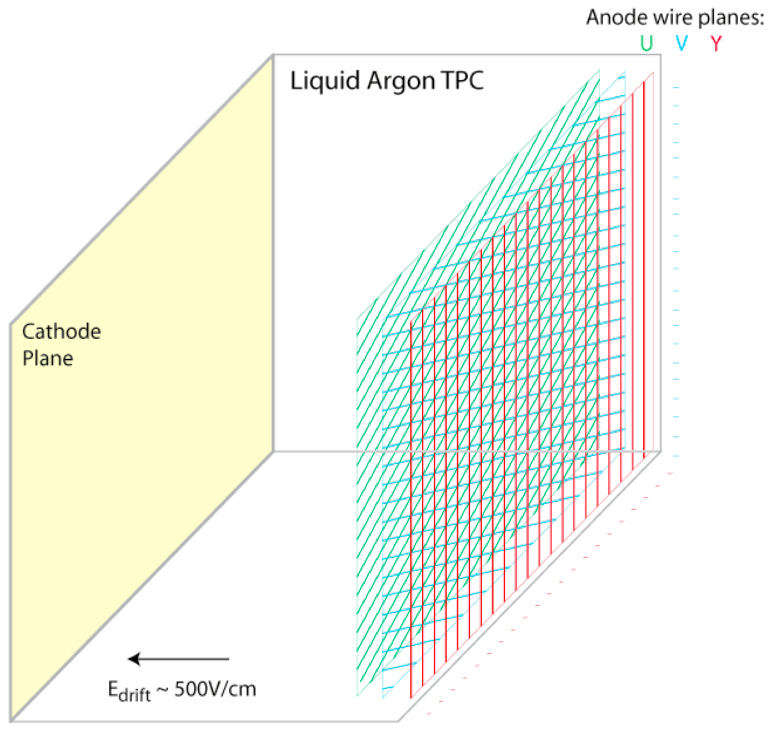
\includegraphics[width=0.98\textwidth]{LArTPCOperation1.png}
    \caption{Typical LArTPC with one cathode (left) and three read out anode planes (right) (two induction, U and V, and one collection, Y), setting up an electric field.  The central region is filled with liquid argon.}
    \label{fig:LArTPCOperation1}
  \end{subfigure}
  \hfill
  \begin{subfigure}[t]{0.48\linewidth}
    \centering
    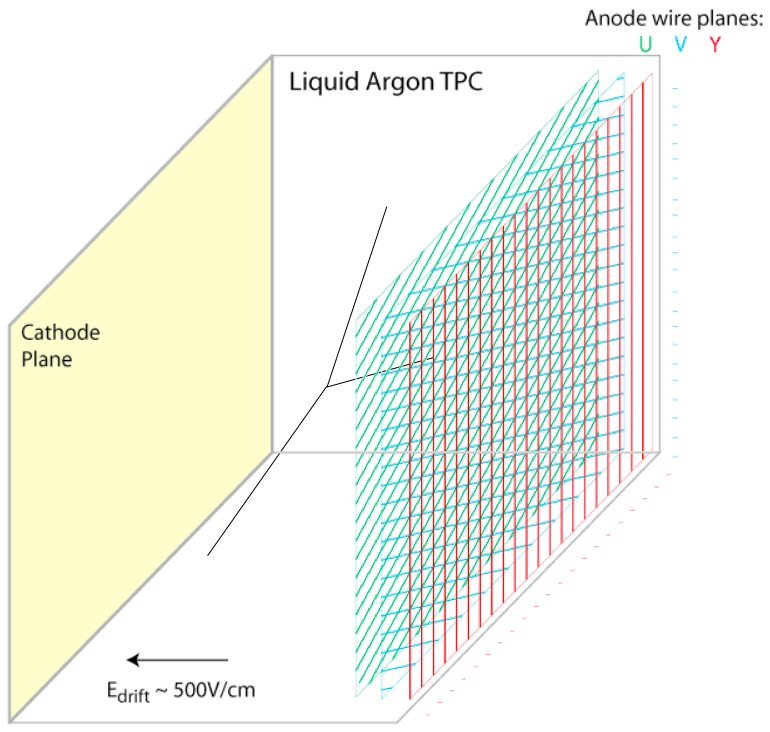
\includegraphics[width=0.98\textwidth]{LArTPCOperation2.png}
    \caption{An ionising particle enters the detector and liberates electrons from the medium, which then drift towards the anode planes.}
    \label{fig:LArTPCOperation2}
  \end{subfigure}
  \hfill
    \begin{subfigure}[t]{0.48\linewidth}
    \centering
    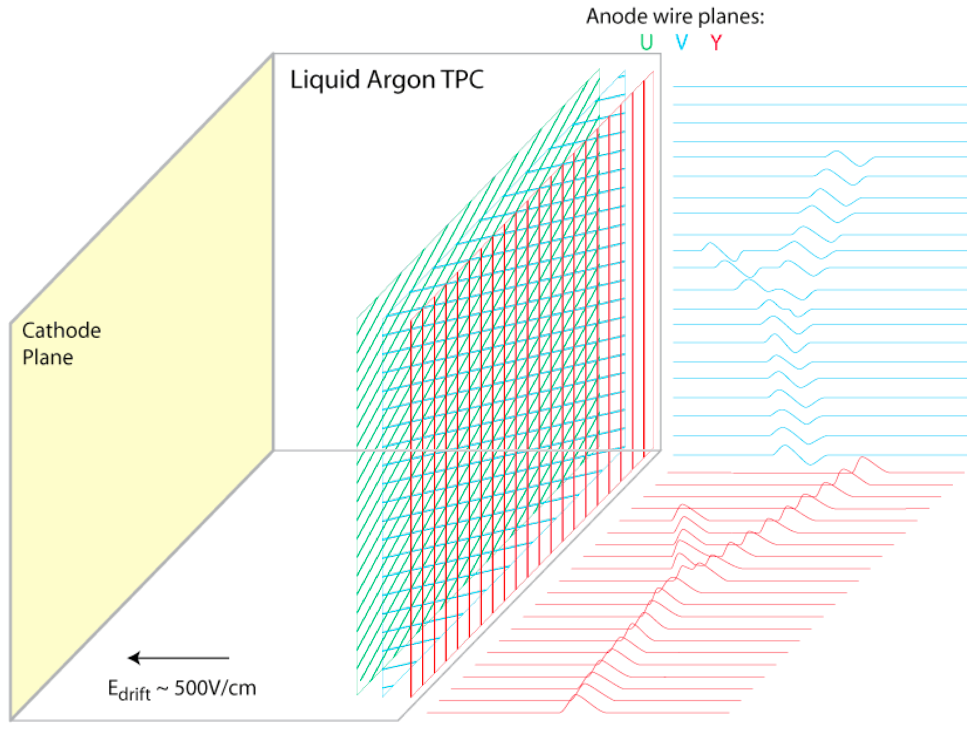
\includegraphics[width=0.98\textwidth]{LArTPCOperation3.png}
    \caption{As the electrons drift through, charge is induced on the first two wire planes and collected on the final one.  Due to the differing orientations of the wires between planes, three complementary views of the interaction are provided (two are shown).}
    \label{fig:LArTPCOperation3}
  \end{subfigure}
  \hfill
  \begin{subfigure}[t]{0.48\linewidth}
    \centering
    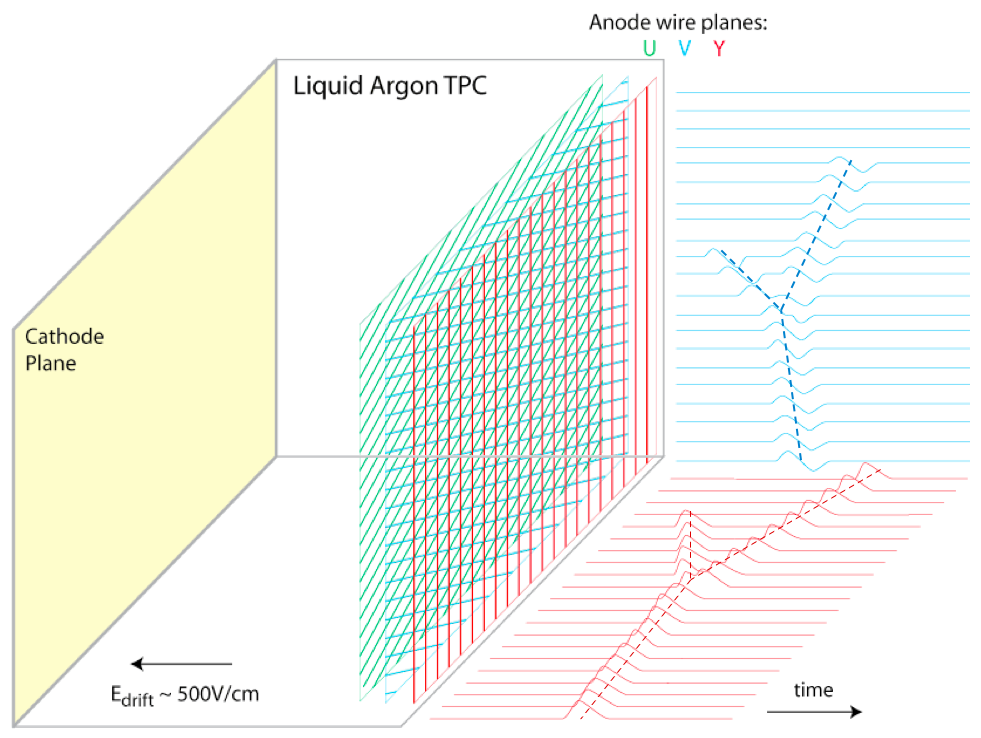
\includegraphics[width=0.98\textwidth]{LArTPCOperation4.png}
    \caption{By combining the two dimensional information provided by the anode planes with the drift time information, the original particle tracks can be inferred.}
    \label{fig:LArTPCOperation4}
  \end{subfigure}
  \caption[Schematic demonstrating the basic operational principles of a LArTPC.]{Schematic demonstrating the basic operational principles of a LArTPC.  The images are stills taken from an illustration created by Bo Yu (BNL) {\color{red}(do I need to cite this?  It's a very common slide and I can't actually find a Bo Yu talk with it in... everyone just puts his name on the slide!)}.}
  \label{fig:LArTPCOperation}
\end{figure}

%----------------------------------------------------------------------------------------------------------------------------------------------------------------------------
\subsection{LArTPC Challenges}\label{sec:LArTPCChallenges}

There is no doubt of the promise of LArTPCs for the future of neutrino physics but with such expectation comes many challenges.  This will be elaborated upon in more detail when discussing the 35~ton run in Section~\ref{sec:35tonPhaseII} but will be briefly mentioned here for completeness.

Given the drift fields required, and the necessary distances, the associated high voltage on the cathode must be on the order of $\sim$100~kV.  This presents engineering challenges related to the feedthrough and cryostat design but also can lead to dielectric breakdown of the liquid nearby such huge voltages.  The properties of LAr and the design implications must be very well understood to ensure this does not endanger the quality of the detector medium.

The presence of electro-negative impurities in the argon can capture drift electrons as they travel towards the anode planes and hinder the signal observed.  The probability of this recombination is referred to as the `electron lifetime' and is directly affected by the maintained purity of the argon.  DUNE expects a contaminant no greater than \#\# ppm O2 and \#\# ppm N2 [to be filled in when I write the DUNE chapter].  This necessitates a purification system to remove impurities and requires the constant recirculation of the liquid through it.  A liquifier is also necessary to recondense any boiled-off gases at the surface.

Along with the possibility of lost signal through finite electron lifetimes, the electrons may also undergo interactions and drift off course either transversely or longitudinally.  This `diffusion' affects the location and size of the observed signal so must also be well understood.

With so much resting on the success of the DUNE experiment, and considering all these effects which must be understood, prototyping is essential.  The 35~ton prototype was constructed as an attempt to better understand LArTPCs and is the subject of Chapter \ref{chap:35ton}.

%----------------------------------------------------------------------------------------------------------------------------------------------------------------------------
\section{Overview of DUNE}\label{sec:DUNEOverview}

The outstanding questions in neutrino physics discussed in Section~\ref{sec:NeutrinoPhysicsStatus}, namely the resolution of the mass hierachy, the determination of the CP-violating phase $\delta_{\textnormal{CP}}$, the measurement of the octant of $\theta_{23}$ and precision calculations of all the mixing angles, motivate the need for next generation experiments.  The DUNE experiment will make decisive contributions to each of these areas; it will also search for nucleon decay with the ability to set world-leading proton lifetime limits and make detailed, unique measurements of the $\nu_e$ flux from a core-collapse supernovae within our galaxy should one occur during the experiment.  Along with this, DUNE will be used to look for Beyond Standard Model physics (such as non-standard interaction and sterile neutrinos), signatures of dark matter and, utilising the capable near detector, measurements of a range of neutrino cross-sections and nuclear effects including final state interations.

The chosen technology for the DUNE far detector, in order to maximise sensitivity to all these factors, is a liquid argon (LAr) TPC (LArTPC), introduced and described in Section~\ref{sec:LArTPC}.  The detector will contain four modules, each comprised of 10~kt fiducial LAr and separate data acquisition and readout systems.  The beam will be provided by Fermilab as part of its PIP-II program \cite{PIPII2013} and will be wide band, enabling the study of a range of neutrino energies.  This facilitates a study of multiple oscillation peaks, essentially due to differing $L/E$ ratios, and is relevant when considering the effects of an unknown CP-violating phase and unresolved mass hierarchy.  Since the impact of both of these uncertainties is apparent as an asymmetry between neutrinos and antineutrinos (Equation \ref{eq:NeutrinoAntineutrinoAsymmetry}), there is an implicit degeneracy which must be resolved to ensure both phenomena are correctly determined.  Having access to multiple oscillation peaks means this may be dealt with in a single experiment, as demonstrated in Figure~\ref{fig:TwoPeakAmbiguity} \cite{Huber2011}.

\begin{figure}
  \centering
  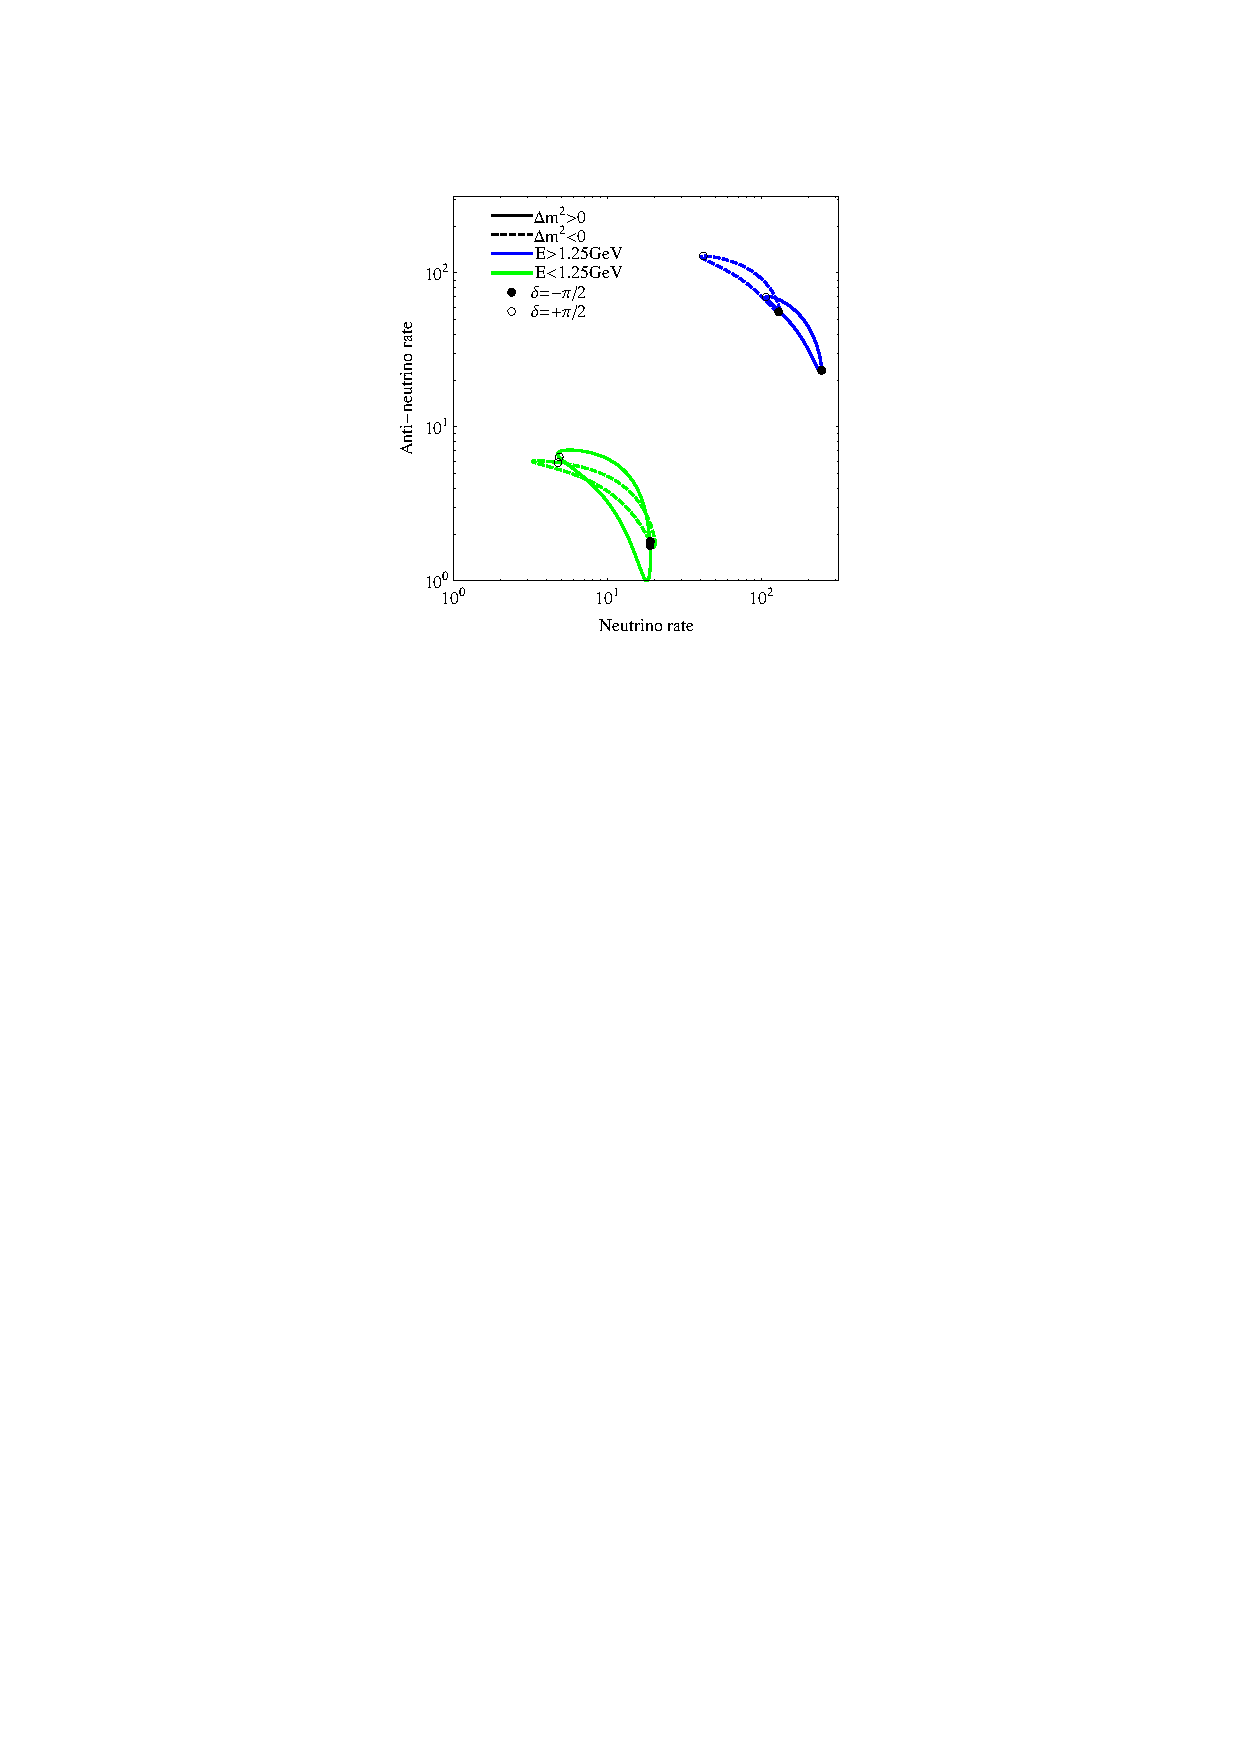
\includegraphics[width=10cm]{TwoPeakAmbiguity.pdf}
  \caption[Demonstration of how having access to multiple oscillation maxima facilitates measurements of both the neutrino mass hierarchy and leptonic CP-violation using the same experiment.]{Demonstration of how having access to multiple oscillation maxima facilitates measurements of both the neutrino mass hierarchy and leptonic CP-violation using the same experiment.  In the plot, $\theta_{13}$ is held constant and the rates are determined by the number of neutrino and antineutrino events respectively.  Assuming a baseline of 1300~km, as for DUNE, the first oscillation maximum is at $E_{\nu}=2.5$~GeV and the second is at $E_{\nu}=0.84$~GeV.  The banana-shaped distributions are obtained as the value of $\delta_{CP}$ is varied from $-\pi$ to $\pi$.  There is good separation between the distributions associated with each hierarchy at the first maximum whereas at the second maximum this is degenerate and the rates are similar for a given value of $\delta_{CP}$ regardless of the hierarchy.  It can be seen how complimentary measurements at each maxima can be used to make unambiguous measurements of both the mass hierarchy and of CP-violation with the same experiment.  Taken from \cite{Huber2011}.}
  \label{fig:TwoPeakAmbiguity}
\end{figure}

DUNE was officially formed in early 2015 following the dissolution and merging of two leading next generation long-baseline experiments: the Long Baseline Neutrino Experiment (LBNE) in the U.S. \cite{LBNECDR1,LBNECDR3,LBNECDR4a} and the Large Apparatus for Grand Unification, Neutrino Astrophysics, and Long Baseline Neutrino Oscillations (LAGUNA-LBNO) in Europe \cite{LAGUNA-LBNO2015}.  Given the scale of these projects, it was decided in 2014 that efforts should be focussed on one flagship experiment utilising the expertise of as many experts in neutrino physics and LArTPC technology as possible \cite{P52014}.  The Particle Physics Project Prioritisation Panel review recommended.......  The benchmark DUNE design is very similar to that of the former LBNE experiment, which also made use of an upgraded Fermilab neutrino beam and a large LArTPC at SURF, and gained the understanding of dual phase LArTPC detectors developed by LAGUNA-LBNO. {\color{red} Need to mention dual phase in the first section.}  It is likely that at least one of the four DUNE detector modules will be a dual phase LArTPC.

The experiment will be facilitated by the Long Baseline Neutrino Facility (LBNF), which will oversee the technical side of the project and ensure the DUNE experiment can function as desired.  The relationship between the LBNF and the DUNE projects is based on the model used at CERN to manage the Large Hadron Collider (LHC) and each of the experiments which use it.  LBNF has its own management structure and operates separately from DUNE, though the two projects work closely together.  It is supported mainly via the Department of Energy in the U.S. whereas DUNE is internationally funded.  The DUNE collaboration is responsible for defining the scientific goals of the experiment and the corresponding techincal requirements.  Using these, LBNF will design and construct all technical facilities, such as the beam upgrade, the facilities for the near detectors at Fermilab and the excavation and outfitting of the large caverns for the far detectors underground at SURF along the required infrastructure to support the construction of the cryostats and the associated cryogenic systems.  DUNE will provide the four massive LArTPCs and the near detector systems, to be constructed at the sites supplied by LBNF.  These will be discussed further in Section~\ref{sec:DUNEExperiment}.  During the lifetime of the experiment, LBNF is responsible for the maintaining and operation of all the facilities whilst DUNE will commission and operate the detectors.  The scientific research program conducted with the collected data is the duty of the DUNE collaboration and will be explored in Section~\ref{sec:DUNEPhysics}.

Given the scale of the projects, work is already underway.  Construction at the far detector site starts this year, with installation of the first detector module due to commence in 2021.  The start of the DUNE experiment will then correspond to the completion of this module, scheduled in 2024.  The PIP-II upgraded 1.2~MW beam will be ready in 2025 and will signify the commencement of beam data taking.  Subsequent detector modules will be added as soon as is feasible thereafter, increasing the fiducial volume up to the target mass of 40~kt.  Further beam upgrades, up to 2.4~MW (PIP-III) are envisaged beyond this to bring the experiment up to full power and maximise the physics capability of the project.  The timescales of both LBNF and DUNE, along with all the essential research which must be conducted as the plans progress, is the subject of Section~\ref{sec:RoadToDUNE}.

%----------------------------------------------------------------------------------------------------------------------------------------------------------------------------
\section{Experimental Details}\label{sec:DUNEExperiment}

%----------------------------------------------------------------------------------------------------------------------------------------------------------------------------
\subsection{Beam}\label{sec:DUNEBeam}

%----------------------------------------------------------------------------------------------------------------------------------------------------------------------------
\subsection{Near Detector}\label{sec:NearDetector}

%----------------------------------------------------------------------------------------------------------------------------------------------------------------------------
\subsection{Far Detector}\label{sec:FarDetector}

%----------------------------------------------------------------------------------------------------------------------------------------------------------------------------
\section{The Physics of DUNE}\label{sec:DUNEPhyics}

The staged approach to the DUNE experiment will allow early preliminary results but will require more time for facilities from later phases to be constructed and commissioned.  For this and other reasons, the accumulated data is often referred to as an `exposure', a function of detector size, beam power and time with units kt$\cdot$MW$\cdot$year.  The current assumptions on exposures for the first few years of operation are shown in Table~\ref{tab:DUNEExposure}.  This staging will be assumed in all sensitivities presented in this section.

\begin{table}
  \caption{Exposures anticipated for the DUNE experiment for the first few years of operation.  Due to the staged approach in construction, it will take some time to reach full design capabilities.  The first exposure column represents the exposure expected in that year and the next column the cumulative total.}
  \label{tab:DUNEExposure}
  \centering
  \begin{tabular}{ >{\raggedright\arraybackslash}m{1.5cm} >{\raggedright\arraybackslash}m{2.5cm} >{\raggedright\arraybackslash}m{2.5cm} >{\raggedright\arraybackslash}m{7cm} }
    \toprule
    Year & Exposure (kt$\cdot$MW$\cdot$year) & Total (kt$\cdot$MW$\cdot$year) & Detector stage \\[1ex]
    \midrule
    Year 1 & 10.7 & 10.7  & 10~kt far detector, no near detector, 1.07~MW 80~GeV proton beam ($1.47\times10^{21}$ pot per year) \\[1ex]
    Year 2 & 21.4 & 32.1  & Addition of second 10~kt far detector module \\[1ex]
    Year 3 & 32.1 & 64.2  & Addition of third 10~kt far detector module and initial constraints from near detector \\[1ex]
    Year 4 & 42.8 & 107.0 & Addition of fourth 10~kt far detector module \\[1ex]
    Year 5 & 42.8 & 149.8 & Inclusion of constraints from full near detector data analysis \\[1ex]
    Year 7 & 85.6 & 278.2 & Upgrate beam power to 2.14~MW for 80~GeV proton beam \\[1ex]
    \bottomrule
  \end{tabular}
\end{table}

The appearance probability expected at the DUNE far detector is demonstrated in Figure~\ref{fig:DUNEAppearanceProbabilities} for various values of $\delta_{CP}$.  

\begin{figure}
  \centering
  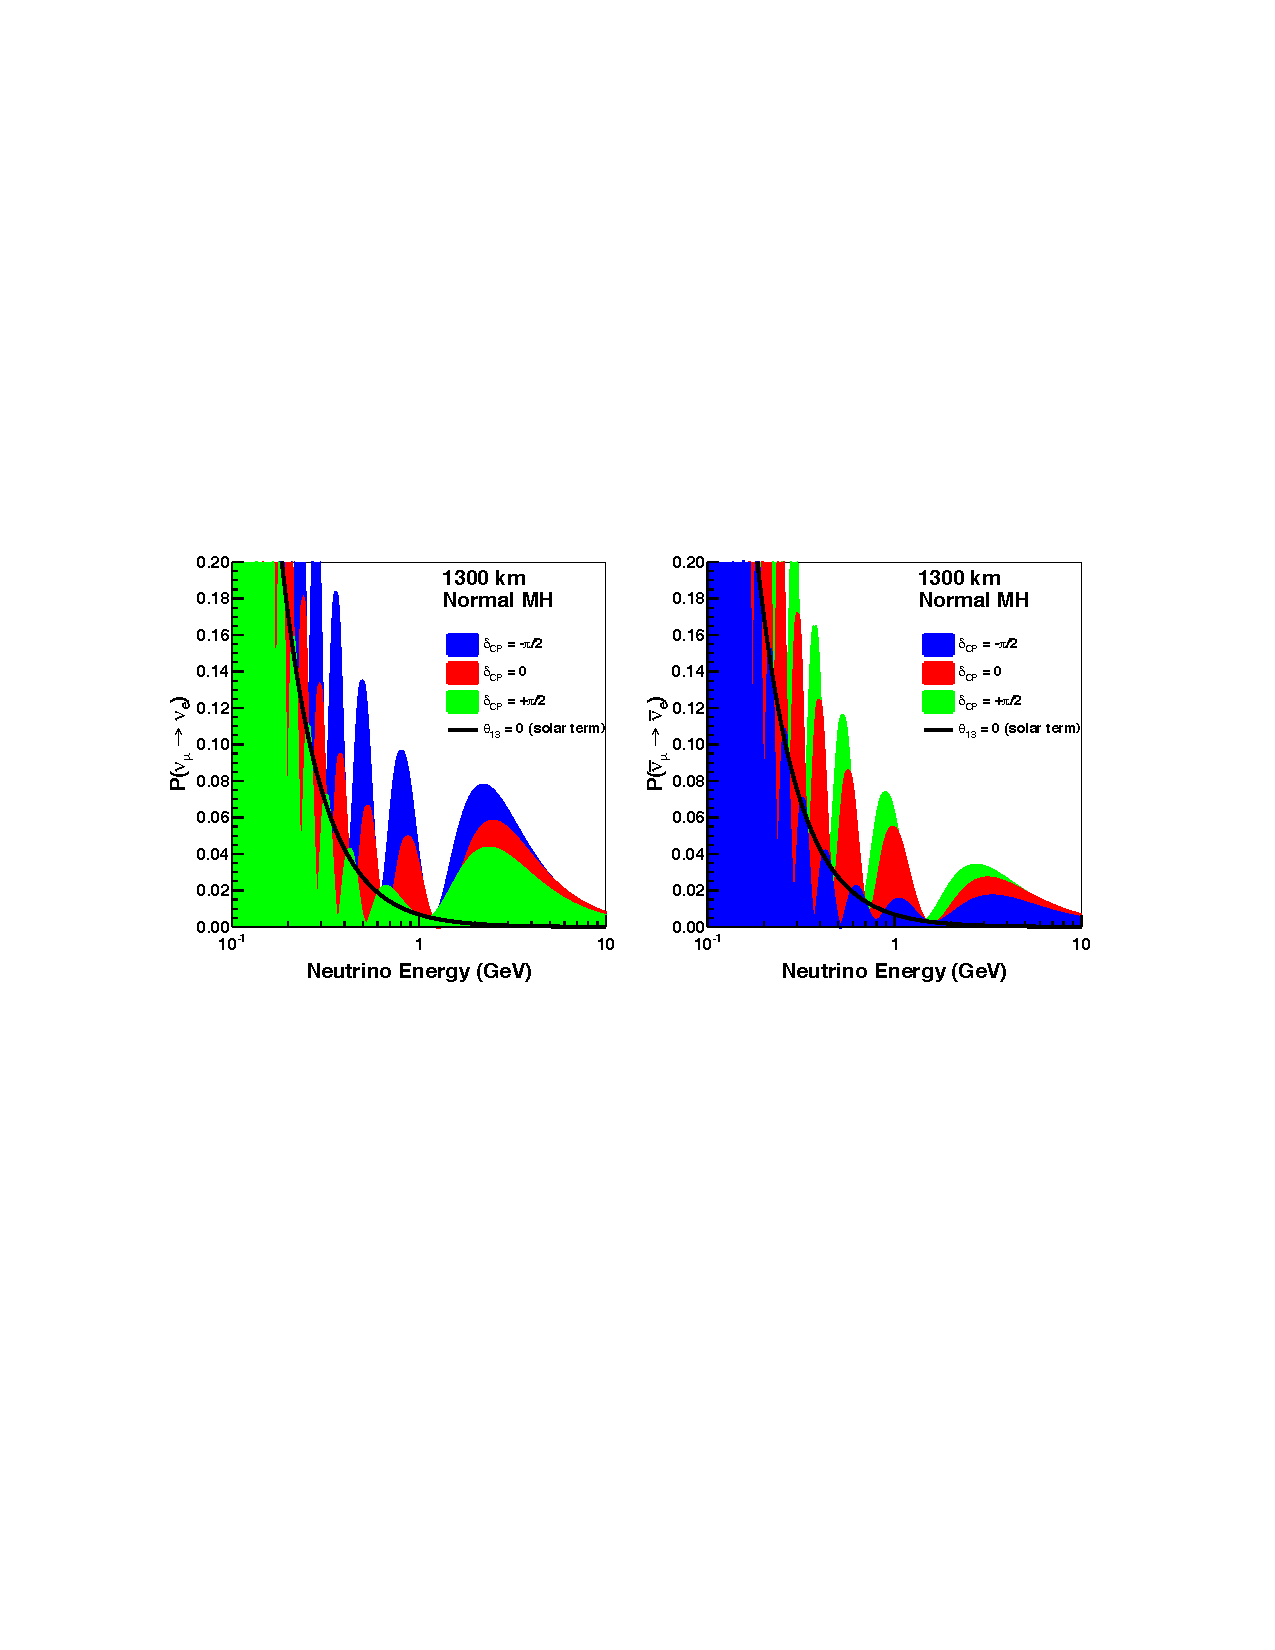
\includegraphics[width=16cm]{DUNEAppearanceProbabilities.pdf}
  \caption{The appearance probability at a baseline of 1300~km, as a function of neutrino energy, for $\delta_{CP}=-\pi/2$ (blue), 0 (red) and $\pi/2$ (green) for neutrinos (left) and antineutrinos (right), for normal hierarchy.  The black lines indicates the oscillation probability if $\theta_{13}$ were equal to zero.  Taken from \cite{DUNECDR2}.}
  \label{fig:DUNEAppearanceProbabilities}
\end{figure}

\subsection{Mass Hierarchy}

The sensitivity of DUNE to the neutrino mass hierarchy is shown in Figure~\ref{fig:DUNEMassHierarchy}.

\begin{figure}
  \centering
  \begin{subfigure}[t]{\linewidth}
    \centering
    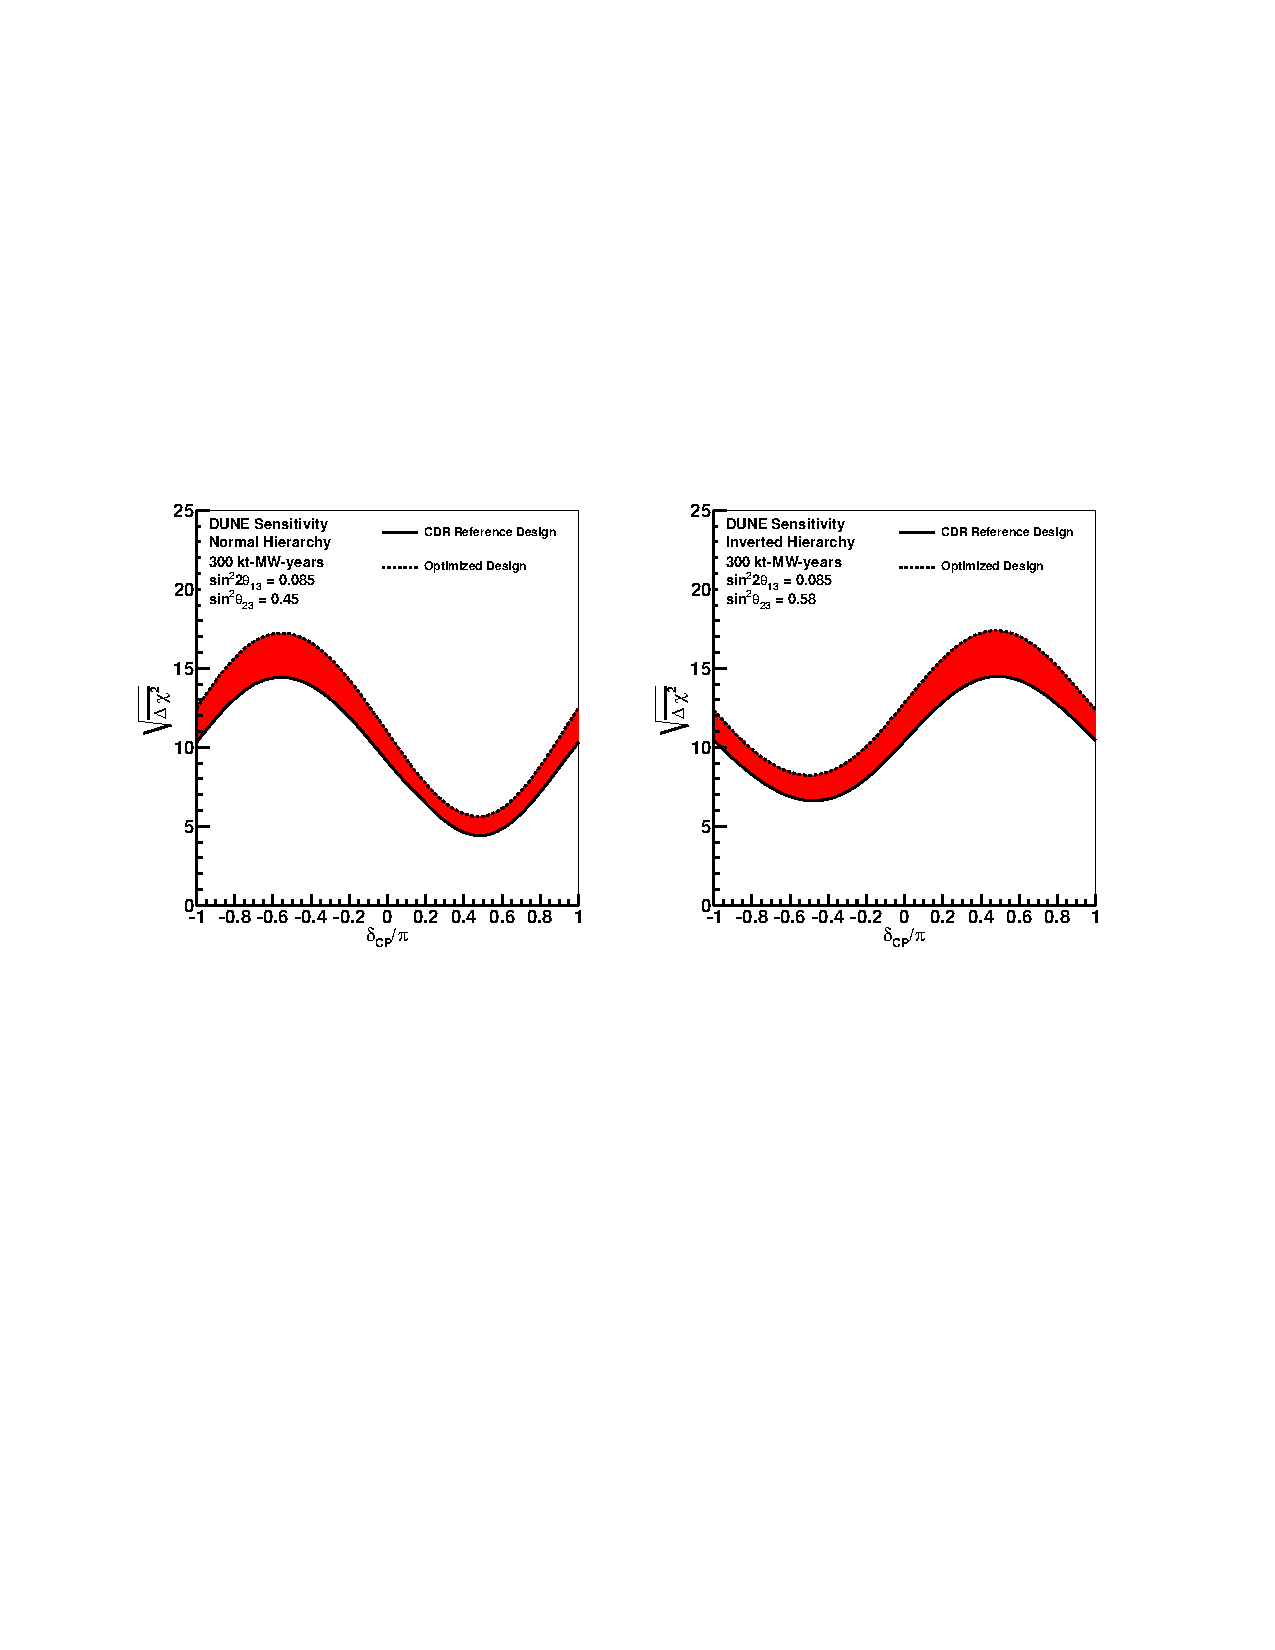
\includegraphics[width=16cm]{DUNEMassHierarchyDeltaCP.pdf}
    \caption{The significance with which the mass hierarchy can be determined as a function of the value of $\delta_{CP}$ for an exposure of 300~kt$\cdot$MW$\cdot$year assuming normal hierarchy (left) and inverted hierarchy (right).  Taken from \cite{DUNECDR2}.}
    \label{fig:DUNEMassHierarchyDeltaCP}
  \end{subfigure}
  \hfill
  \vfill
  \begin{subfigure}[t]{\linewidth}
    \centering
    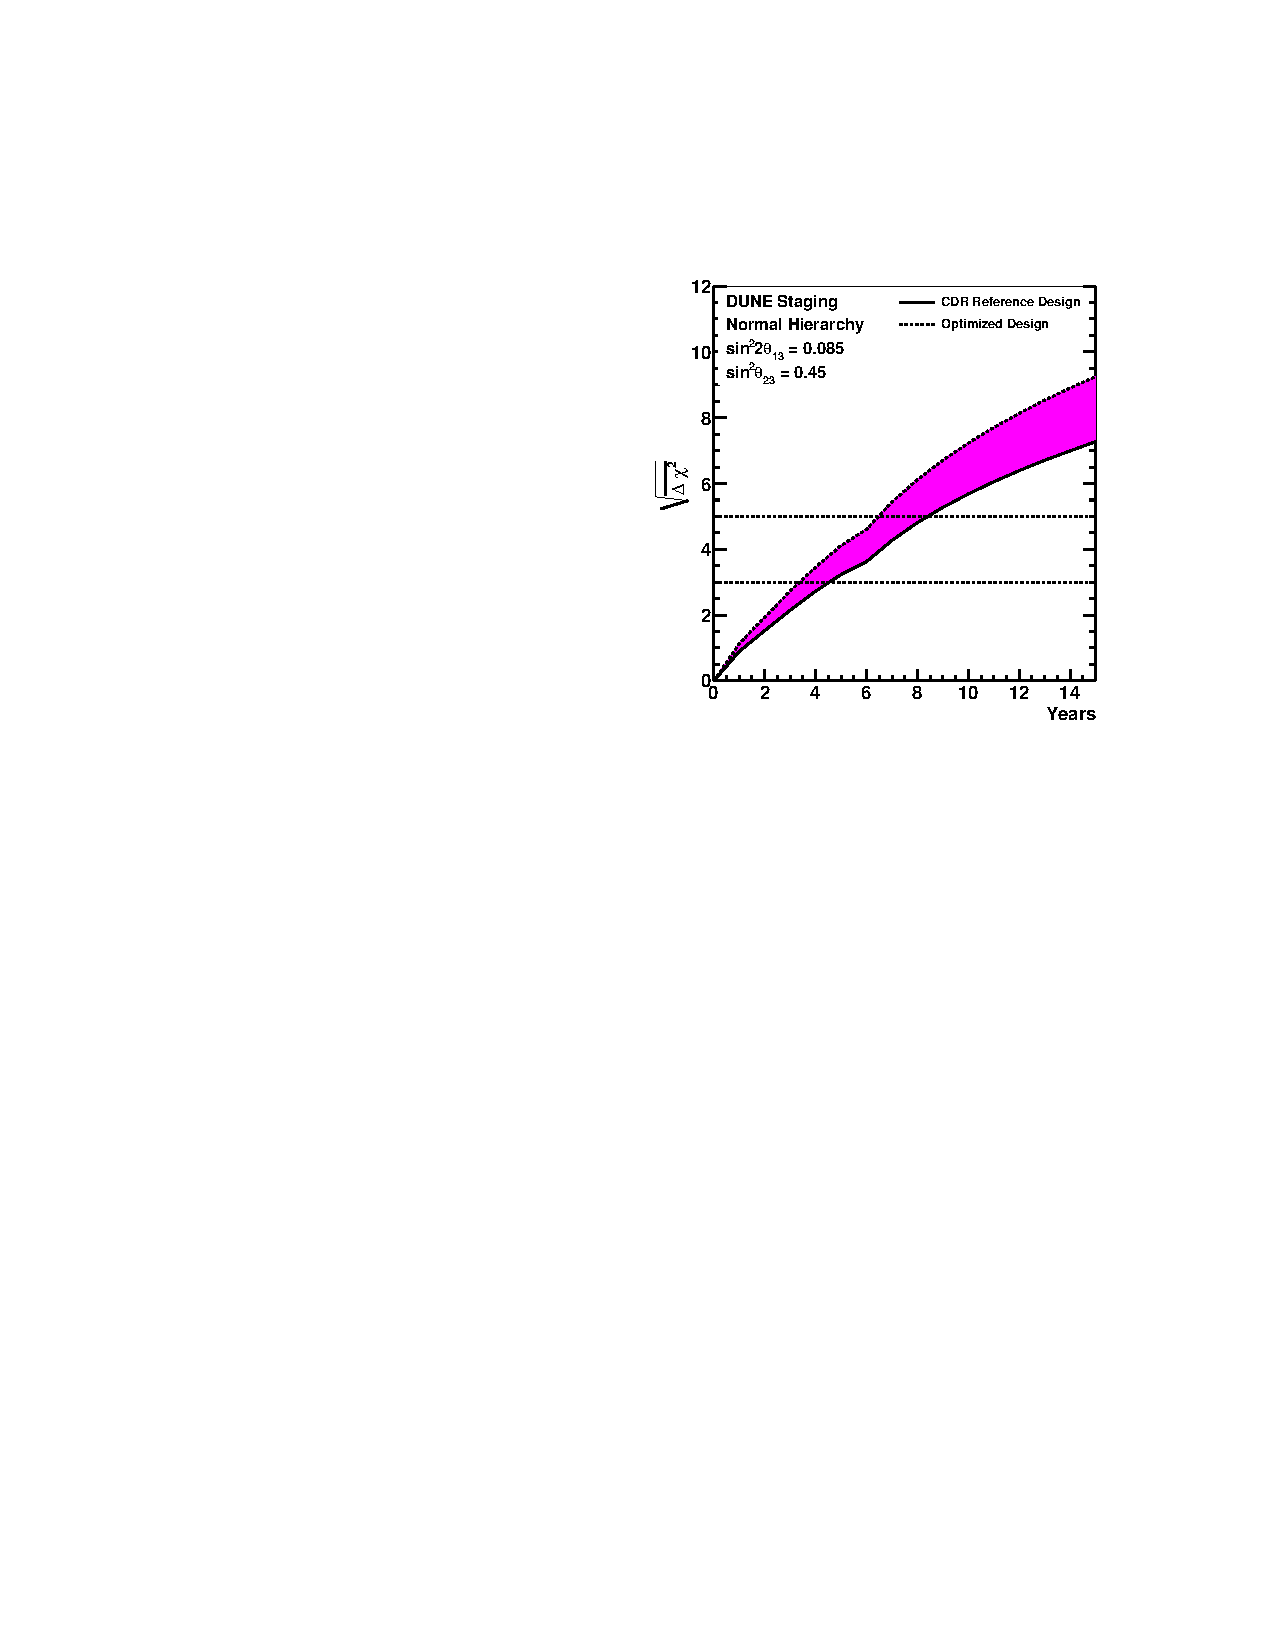
\includegraphics[width=8cm]{DUNEMassHierarchyTime.pdf}
    \caption{Assuming normal hierarchy, the minimum significance (the lowest point on the curve in Figure~\ref{fig:DUNEMassHierarchyDeltaCP}) with which the mass hierarchy can be determined for all values of $\delta_{CP}$ as a function of years of running under the assumptions in Table~\ref{tab:DUNEExposure}.  Taken from \cite{DUNECDR1}.}
    \label{fig:DUNEMassHierarchyTime}
  \end{subfigure}
  \caption[Sensitivity of the DUNE experiment to the neutrino mass hierarchy.]{Sensitivity of the DUNE experiment to the neutrino mass hierarchy.}
  \label{fig:DUNEMassHierarchy}
\end{figure}

%----------------------------------------------------------------------------------------------------------------------------------------------------------------------------
\section{The Road to DUNE}\label{sec:RoadToDUNE}
